%%%%%%%%%%%%%%%%%%%%%%%%%%%%%%%%%%%%%%%%%%%%%%%%%%%%%%%%%%
%
% Vzor pro sazbu kvalifikační práce
%
% Západočeská univerzita v Plzni
% Fakulta aplikovaných věd
% Katedra informatiky a výpočetní techniky
%
% Petr Lobaz, lobaz@kiv.zcu.cz, 2016/03/14
%
%%%%%%%%%%%%%%%%%%%%%%%%%%%%%%%%%%%%%%%%%%%%%%%%%%%%%%%%%%

\documentclass[czech,SP]{thesiskiv}
\author{Jan Pelikán}
\declarationmale

% Název práce
\title{Generátor konečného automatu}

\titlepageyear{\today}

%%%%%%%%%%%%%%%%%%%%%%%%%%%%%%%%%%%%%%%%%%%%%%%%%%%%%%%%%%
%
% DODATEČNÉ BALÍČKY PRO SAZBU
% Jejich užívání či neužívání záleží na libovůli autora 
% práce
%
%%%%%%%%%%%%%%%%%%%%%%%%%%%%%%%%%%%%%%%%%%%%%%%%%%%%%%%%%%

% Umožňuje vkládání obrázků
\usepackage[pdftex]{graphicx}

% Odkazy v PDF jsou aktivní; navíc se automaticky vkládá
% balíček 'url', který umožňuje např. dělení slov
% uvnitř URL
\usepackage[pdftex]{hyperref}
\hypersetup{colorlinks=true,
  unicode=true,
  linkcolor=black,
  citecolor=black,
  urlcolor=black,
  bookmarksopen=true}

% Při používání citačního stylu csplainnatkiv
% (odvozen z csplainnat, http://repo.or.cz/w/csplainnat.git)
% lze snadno modifikovat vzhled citací v textu
\usepackage[numbers,sort&compress]{natbib}
\usepackage{tocloft}
\renewcommand{\cftchapleader}{\cftdotfill{\cftdotsep}} % for chapters
%%%%%%%%%%%%%%%%%%%%%%%%%%%%%%%%%%%%%%%%%%%%%%%%%%%%%%%%%%
%
% VLASTNÍ TEXT PRÁCE
%
%%%%%%%%%%%%%%%%%%%%%%%%%%%%%%%%%%%%%%%%%%%%%%%%%%%%%%%%%%
\begin{document}
%
\maketitle
\tableofcontents

\chapter{Analýza úlohy}
{Jako hlavní problém, který zadání přináší bych nazval naprogramováním konzolové aplikace. Tento problém se dá dekomponovat do menších problémů, jako například: čtení ze souboru, generování kódu či implementace vygenerovaného kódu.}\\
{Začněme tedy čtením ze souboru, to lze realizovat pomocí funkcí \textit{fgetc()} nebo \textit{fgets()}. Použitím první zmíněné funkce budeme číst znak po znaku a použitím druhé funkce lze číst celou řádku až v souboru. Jak lze vidět na ukázce níže, na každé řádce se nachází pouze jedna podstatná informace, tudíž jsem pro svoji implementaci zvolil druhou možnost (\textit{fgets()}). Soubor má vždy stejnou strukturu, tudíž není problém se čtením různých souborů a obecné předpoklady jsou vždy splněny.} 
\begin{figure}[!ht]
\centering
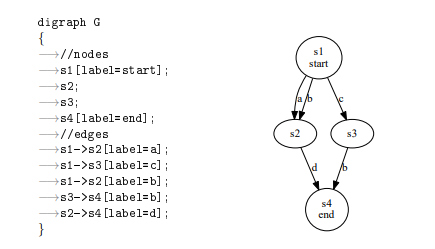
\includegraphics[width=\textwidth]{ukazka_zadani.png} 
\caption{Ukázka ze zadaní}
\label{ukazka}
\end{figure}
{Nastává ale další problém, kterým je získání pouze podstatných informací a oddělení je od zbytku řádky. Důležité informace pro mě jsou: název vrcholu (s1), a pokud má, tak jeho label (start), u hrany jsou důležité informace z jakého a do jakého vrcholu vede a také její label. Jelikož budeme načítat celou řádku, přicházejí v úvahu již implementované funkce pro práci se "stringem". Jedná se o funkce \textit{str...}, které se mohou využít pro rozdělení řádku do příslušných tokenů nebo vyhodnocení, zda se v zadaném řetězci nachází nějaký hledaný řetězec.}\\
{Dále bych zkusil analyzovat problém implementace. Tohle byl pro mě dlouho neřešitelný problém. Nevěděl jsem, jak načtená data uchopit, a jak celý soubor vytvořit. První problém byl vymyšlení vlastní struktury. Možným řešením bylo udělat strukturu grafu, která by uchovávala všechny informace o vrcholech a hranách. Určitě je toto řešení realizovatelné, ale mě se nepovedlo. Místo toho mě napadlo vyřešit problém pomocí dvou struktur, které na sebe odkazují. Další výzvou bylo udělat funkce, které by celý graf zprovoznili. Jednou možností bylo mít jeden generovaný soubor, ve kterém budou funkce pro správu grafu a na konci bude funkce main. Při programování jsem náhodou narazil i na další způsob řešení implementace. Funkce budou v jiném souboru a při pozdějším generování souboru ušetřím drobet času. Využil jsem tedy konstrukci \textbf{\#include <file>}.}\\
{Posledním problémem, který jsem ještě nezmiňoval, bylo generování souboru. K zápisu do souboru lze využít funkci \textit{fputs()}, která zapisuje do souboru. Napadají mě dvě možnosti řešení. Jednou z možností je vytvoření si jednoho velkého bufferu (pole znaků) a zapisování do něj a druhou možností je postupné zapisování do souboru (využití více metod fputs). Zvolil jsem druhou možnost, protože jsem se vždy postupně "zbavoval" potřebného textu k vygenerování.}

\chapter{Popis implementace}
{Jako první budu popisovat implementaci generátoru. Generátor je implementován jako jeden soubor \textbf{fsmgen.c}. Nejdříve jsem implementoval funkce, které později využívám v mainu. První funkcí je \texttt{odstran\_tab(char* vstup)}. Tato funkce se využívá při generování souboru fsm.c a slouží pro odstranění tabulátoru nebo mezer ze začátku načtené řádky (viz "--->"  na obrázku \ref{ukazka}). Další dvě funkce (\texttt{introInfo() a inputInfo()}) jsou pouze pro vypisování informací pro uživatele. Zajímavější funkce už jsou \texttt{pridej\_vrchol(char[] radka) a pridej\_hranu(char[] radka)}. Obě funkce fungují na podobném principu. Rozdílné jsou jen v tom, zda v zadaném parametru najdeme informace o vrcholu či hraně. Funkce potom řádku ořezají abych dostal pouze podstatné informace. Využívám funkce \texttt{strtok(char *str, const char *delim)}, která rozděluje vstup podle zadaného rozdělovače. Toho využívám k získání názvů vrcholů a labelů. Funkce vrací předpřipravený řetězec, který je připravený pro zápis do generovaného souboru (validní ANSI C kód). Poslední funkcí v souboru je funkce main. Zde zkontroluji vstupní parametry a buďto program pokračuje se zadaným vstupem, nebo se program ukončí a vypíše hlášku v angličtině uživateli. Poté se otevřou soubory a začne čtení souboru. Jako první se přečtou 3 řádky ze souboru, to jsou řádky, které neobsahují žádné důležité informace. Poté začne while cyklus přes všechny řádky souboru, pokud je na zadané řádce \textit{//edges} tak program skočí do vnitřního cyklu, kde přidává hrany. Pokud se narazí na konec souboru z obou while cyklů se vyskočí. Implicitně se do generovaného souboru jako první přidávají vrcholy a poté až hrany. Při dokončení čtení ze souboru dopíšu do generovaného souboru konec a zavřu všechny soubory. Nakonec vypíšu hlášku o úspěšném provedení.} \\ 
{Jako další krok bych popsal implementaci generovaného souboru. Soubor jako takový obsahuje pouze jednu funkci a to je funkce main. Další funkce se přidávají pomocí \textbf{\#include} z dvou dalších souborů. Na začátku funkce pouze zkontroluji vstupní parametry. Pokud je zadán pouze jeden parametr, proběhne zbytek programu, to znamená, přidají se všechny vrcholy a hrany do seznamu vrcholů. Po přidání všech hran a vrcholů se zkontroluje vstupní řetězec a uživatel se informuje o správnosti/nesprávnosti jeho vstupu. Soubor buďto skončí jako \textit{EXIT\_SUCCES} nebo \textit{EXIT\_FAILURE} a vždy se z paměti vyčistí všechny alokované rámce paměti. Funkce, které tento soubor, využívá jsou v souborech \textit{fsm\_sprava.c} a \textit{fsm\_pridani.c}. Tyto soubory "includuji" hned na začátku souboru.}\\
{První soubor, který bych popsal, je \textit{fsmgen.h}, v tomto souboru deklaruji svoje dvě struktury. Strukturu hrana a strukturu vrchol. Podíváme se na tyto struktury blíže. Struktura vrchol obsahuje jméno a label vrcholu, počet hran, které jsou k vrcholu připojeny a dále odkazuje na následující vrchol (takový spojový seznam) a pole hran (odkaz na strukturu hrany). Struktura hrany obsahuje názvy obou svých vrcholů, svůj label a také odkaz na další vrchol neboli vrchol do kterého hrana vede.}
\begin{figure}[!ht]
\centering
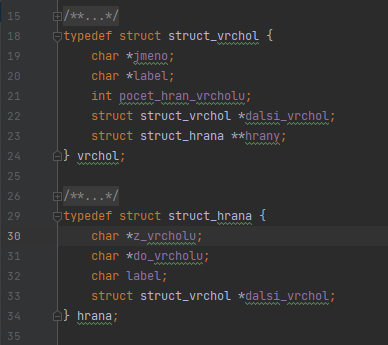
\includegraphics[width=\textwidth]{struct.png} 
\caption{Ukázka použitých struktur}
\label{struct}
\end{figure}
\\{Dalším v pořadí je soubor \textit{fsm\_sprava.c}. V tomto souboru řeším uvolňování paměti a kontrolu vstupu. Funkce \texttt{free\_vsechno(vrchol* vrcholy)} není ničím zvláštní. Jako parametr předávám pole vrcholů, které postupně čistím. Nejdříve uvolním všechny hrany, potom uvolním pole hran a nakonec i celý vrchol. Využívám zde spojového seznamu v posunu na další vrchol. Funkce \texttt{zkouska\_grafu(vrchol* vrchol)} kontroluje, zda se v zadaném seznamu nachází vrchol, který by měl label start. Pokud label start najde, vrací 1 (true). Této funkce využívám ve funkci \texttt{zkouska\_vstupniho\_retezce(char *retezec, vrchol *vrchol)}, tato funkce prochází celý řetězec a porovnává znak po znaku s labelem každé hrany a pokud se rovnají, posunuje se na další vrchol dané hrany. Pokud se shodná hrana nenajde, program končí chybou a vypsáním chybového hlášení. Pokud celý řetězec projde úspěšně, tak se na konci vyhodnotí, zda koncový bod má label "end" nebo ne. Tudíž jestli jsme došli do cíle nebo ne.}\\
{Posledním souborem je \textit{fsm\_pridani.c}, v tomto souboru jsou funkce pro přidání hrany a vrcholu. Funkce pro přidání vrcholu v parametrech obdrží seznam již vytvořených vrcholů, svůj budoucí název a label. Na začátku si alokujeme pamět pro daný vrchol, naplním počátečními hodnotami, poté alokuji pamět ještě pro pole hran daného vrcholu. Poté jen procházím seznam a hledám poslední vrchol, když najdu poslední vrchol seznamu, tak přiřadím nově vytvořený vrchol na konec. Funkce pro přidání hrany funguje obdobně ale s menšími úpravami. Po přiřazení vstupních parametrů do struktury začnu prohledávat seznam vrcholů a hledám vrchol, ze kterého hrana vychází. Když najdu, zvýším vrcholu počet hran o 1 a realokuji pamět, poté jen vrcholu přiřadím hranu. Poté už jen v seznamu najdu do kterého vrcholu hrana vede a to je "dalsi\_vrchol" té hrany.}

\chapter{Uživatelská příručka}
{Samotný program pro generování se podle zadání spustí příkazem \textbf{make}. Tento příkaz vytvoří spustitelný soubor \textbf{fsmgen.exe}. Dále už lze spustit program fsmgen s jedním povinným parametrem a tím je název souboru s daty (definicí grafu). Pokud proběhne všechno v pořádku, tak se vygeneruje soubor fsm.c. Tento soubor už si bohužel budete muset ručně přeložit pomocí vašeho překladače. Například příkazem }\\ \\
\texttt{gcc fsm.c -o fsm} \\ \\
{A poté spustit program fsm.exe s jedním argumentem, kterým je cesta po hranách grafu. Program poté vypíše, zda zadaný řetězec úspěšně prošel grafem či ne.}


\chapter{Závěr}
{Musím říci, že před začátkem práce na semestrální práci jsem byl celým jazykem C zmaten a nedokázal si představit, že dokážu něco naprogramovat. Většina práce byla vymýšlení toho, kam mám přidat a naopak kde ubrat * neboli pointer. (Těším se na zkoušku, která mi ukáže, jestli jsem se něco naučil nebo bez stackoverflow nedám ani ránu.) Celá semestrální práce mi dost pomohla v tom uvědomit si, jak by asi programování v ANSI C mohlo vypadat. A ukázalo mi, že jazyk C asi nebude ta správná cesta. Ale celou práci bych hodnotil kladně. Semestrální práce splnila moje očekávání na výbornou. Se svojí prací jsem spokojen i když určitě není ideálně řešená a mohla by fungovat lépe. Myslím si, že zadání jsem splnil správně.  }


\end{document}
